\documentclass[11pt]{report}

\usepackage[portuguese]{babel}
\usepackage[utf8]{inputenc}
\usepackage{graphicx}
\usepackage{hyperref}
\usepackage{indentfirst}
\usepackage{kantlipsum}
\usepackage{float}
\usepackage{listings}
\usepackage{mathtools}
\usepackage{amsmath}
\usepackage{url}
\usepackage[margin=0.8in]{geometry}
\usepackage{biblatex}
\usepackage{multirow}
\usepackage{fancyhdr}
\usepackage[table,xcdraw]{xcolor}
\bibliography{biblio.bib}

\lstset{language=Prolog}

\hypersetup{
    colorlinks=true,
    linkcolor=black,
    citecolor=black,
    filecolor=black,
    urlcolor=black
}

\newlength{\normalparindent}
\setlength{\normalparindent}{\parindent}
\setlength{\parindent}{\normalparindent}

\newcommand{\blank}[1]{\hspace*{#1}}

\renewcommand{\headrulewidth}{0pt}

\pagestyle{fancy}
\fancyhf{}
\rhead{
\includegraphics [scale=0.5]{uproject_new_2.png}}
\rfoot{\thepage}

\begin{document}

\thispagestyle{empty}

\begin{center}
	
	
\includegraphics [scale=0.5]{uplogo500.png}
	\linebreak \linebreak \linebreak \linebreak \linebreak
	\linebreak \linebreak \linebreak \linebreak \linebreak
	\begin{Huge}
		\textbf{U.Project Website} \linebreak \linebreak
	\end{Huge}
	\begin{Large}
		\textbf{Relatório de Estágio} \linebreak \linebreak
	\end{Large}
	\linebreak
	\linebreak
	\linebreak
	\linebreak
	\linebreak
	\linebreak
	Orientadores:
	\linebreak
	\linebreak
	Bruno Fernando Reis Ribeiro Silva - \href{mailto: brunosilva@uproject.pt}{\texttt{brunosilva@uproject.pt}}
	\linebreak
	Márcio Filipe Vilela Fontes - \href{mailto: marciofontes@uproject.pt}{\texttt{marciofontes@uproject.pt}}
	\linebreak
	\linebreak
	\linebreak
	\linebreak
	UPTEC - Parque de Ciência e Tecnologia da Universidade do Porto
	\linebreak
	Rua Alfredo Allen, nº455/461, 4200-135 - Porto, Portugal
	\linebreak
	\linebreak
	\linebreak
	\linebreak
	5 de Setembro de 2015
\end{center}

\newpage

\pagenumbering{roman}

\chapter*{Agradecimentos}
\addcontentsline{toc}{chapter}{Agradecimentos}
Agradecemos ao Bruno Silva e ao Márcio Fontes pelo esforço e dedicação em nos ensinarem as coisas necessárias para a realização deste projeto e pelo apoio nas nossas dificuldades.
\newpage

\chapter*{Sumário}
\addcontentsline{toc}{chapter}{Sumário}
Neste relatório encontra-se um resumo do que foi realizado na empresa U.Project durante a realização dos capitulos A2-A4.
\newpage

\chapter*{Abstract}
\addcontentsline{toc}{chapter}{Abstract}
This report is a summary of what was accomplished in U.Project during 4 days, between the sections A2 and A4.
\tableofcontents

\newpage

\pagenumbering{arabic}

\newpage

\chapter{Introdução}

\section{Descrição}
Nesta semana inicial da Fase Final de estágio foi-nos pedido que fizéssemos uma proposta de website, responsivo e de fácil utilização e manutenção, para a U.Project. /linebreak
Fomos divididos em 3 equipas, cada equipa composta por 2 elementos, com o objetivo de nos organizarmos com mais facilidade. /linebreak
O nosso trabalho foi organizado com um diagrama de Gantt o que, sem dúvida, nos facilitou o trabalho realizado até hoje. /linebreak
Para descrever o trabalho desenvolvido, realizamos este relatório.
\section{Objetivos}
O objetivo deste relatório é descrever o trabalho realizado, nos quatro primeiros dias da Fase Final deste estágio, no website para a U.Project (A2-A4).
\section{Estrutura do Relatório}
O relatório está dividido em titulos e sub-titulos, começando por uma introdução, seguindo por empresa e o projeto realizado e finalizando com opiniões dos estagiários.
\chapter{A Empresa}

\section{Caraterização da Empresa}
A U.Project é uma organização com a missão de potenciar e impulsionar o empreendedorismo jovem. Para isso, atua em duas frentes vitais para permitir às Startups criar e desenvolver as suas ideias que, de outro modo, seriam praticamente impossíveis de serem concretizadas devido aos custos e desafios envolvidos no processo.

Em primeiro lugar pretende, através da U.Project Startup Network, oferecer diversos modelos de contrato adaptados a cada Empresa de modo a que estas tenham acesso aos recursos e serviços necessários ao seu desenvolvimento.

Em segundo lugar acompanha e orienta, através da U.Project Academy, os alunos desde o ensino secundário, de modo a potenciar e desenvolver as suas capacidades para poderem participar no desenvolvimento de novos projetos e ideias. Através de um programa de estágio, em parceira com as respetivas escolas, os alunos têm acesso a diversas formações e atividades, além de terem a possibilidade de integrar uma equipa de desenvolvimento.

Para além de fornecer os seus serviços, a U.Project pretende também criar uma rede interna de empresas, de modo a que estas possam encontrar de uma forma fácil e rápida os serviços que necessitam, através do produto de outras pertencentes à rede, permitindo assim a realização de melhores negócios e um aumento na divulgação das mesmas.

Os associados da organização podem usufruir de diversos serviços e formações através do pagamento de uma quota. Quem achar que possui os requisitos necessários para trabalhar a tempo inteiro pode candidatar-se a membro, trabalhando diretamente para a empresa e usufruindo de um salário fixo de acordo com a posição ocupada, podendo também ser promovido pela direção a um cargo superior.

Quando um membro ultrapassar os 30 anos, pode ser premiado com o título de membro honorário, ficando isente do pagamento de quotas e passando a ter funções de aconselhamento e divulgação.

\section{Objetivos da Empresa}
A U.Project tem como objetivo promover o epreendedorismo jovem, dando apoio às Startups, para que estas se consigam desnevolver sem terem a necessidade de possuir vastos recursos financeiros.
Para isso a U.Project irá acompanhar os jovens desde o ensino secundário, apoiando-os e orientando-os na vida Universitária através da realização de estágios, competições, atividades,...
Também irá estimular e incentivar estes alunos a desenvolverem as suas ideias e projetos, aproximando-os das Startups, fomentando assim o emprego jovem e granatindo um acompanhamento ao desenvolvimento dos seus projetos.

\section{Historial da Empresa}

\section{Estrutura Hierárquica}

Direção
\begin{itemize}
\item Presidente - Bruno Silva
\item Vice-Presidente - Márcio Fontes
\item Secretário - José Coutinho
\end{itemize}
Departamento de Comunicação e Imagem
\begin{itemize}
\item Catarina Reis
\item João Marques
\item Jorge Loures
\item Rita Cardoso
\item Tatiana
\end{itemize}
Conselho Científico
\begin{itemize}
\item Nuno Flores
\end{itemize}

\section{Áreas de Negócio}
A U.Project fornece recursos às Startups interessadas em começar o seu negócio no mundo Empresarial, permitindo assim uma redução significativa nos seus custos.
Também atua no mundo académico, acompanhando os alunos desde o ensino secundário, orientando-os e ajudando-os a integrarem-se no mundo profissional, fornecendo-lhes pelo caminho diversas aptidões e conhecimentos essenciais em diversas áreas.
\section{Logótipo}
\begin{center}

\includegraphics [scale=0.5]{uplogo500.png}
\end{center}
\section{Localização}
\textbf{UPTEC - Parque de Ciência e Tecnologia da Universidade do Porto} 


Morada:
Rua Alfredo Allen, n.º455/461
4200-135 Porto


GPS:
+41º 10'38,89'' N, -8º 36'18,25'' O


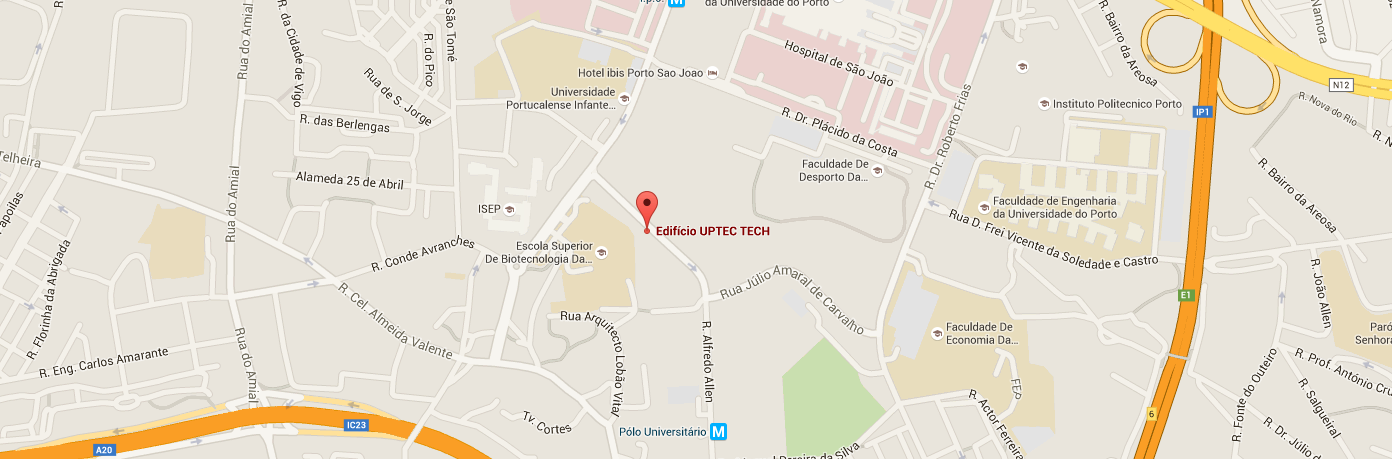
\includegraphics [scale=0.35]{location.png}

\newpage

\chapter{O Projeto}
\section{Descrição}
O projeto consiste na realização de um website para a U.Project. Este é constituído por duas partes: uma pública e outra privada.
A seccção pública do website permite dar a conhecer a orgaização aos visitantes, desde os objetivos, descrição e projetos até às diversas atividades organizadas por ela.
A outra parte do website apenas se encontra acessível aos associados e membros da U.Project. Aqui, os membros podem editar as suas informações pessoais, regularizar as suas quotas e comunicar com outros utilizadores.
Os membros podem também gerir os seus trabalhos e projetos.
A direção tem acesso ao painel de administração que permite o controlo total do website desde páginas, utlizadores,eventos, pagamentos, finanças e departamentos.
O administrador do website garante que este se encontra em funcionamento e que todos cumprem as regras de utilização do mesmo.
\section{Objetivos}
O objetivo deste projeto é criar um website de fácil utilização e manutenção para a empresa U.Project e que permita o log in no website assim como o registo no mesmo e tambem a possibilidade de inscrever nas atividades.
\section{Funcionalidades}
Formulário de Contacto;
Newsletter;
Interação com redes sociais;
Acesso restrito ao login;
Painel administrativo com possibilidade de alterar qualquer página;
Slideshow na página inicial;
Página de notícias;
Página de eventos a decorrer e eventos futuros;
Interação com o google maps;
Interação com os departamentos e possibilidade de se inscrever.
\section{Ferramentas a utilizar}
Utilizamos o Architect Enterprise que é uma ferramenta de modelagem e design. Esta plataforma suporta a concepção e construção de sistemas de software.
Tambem utilizamos o photoshop para criar prototipos do layout do website.
\section{Atividades a desenvolver}

\section{Calendarização do Projeto}

\section{Fases de Implementação}
3.7 Fases de Implementação
	3.7.1 Actors e User Stories
Começamos por criar os Actors, que é um diagrama em que cada pessoa representa uma pessoa, organização ou sistema externo que pode interagir com o sistema definindo assim as suas permissões.
https://scontent-mad1-1.xx.fbcdn.net/hphotos-xat1/v/t34.0-12/10617786_879407858807290_488390428_n.jpg?oh=de2ff8ec757f5e2b5bcf3b1da0f5da54&oe=55EF32A6
De seguida fomos para os User Stories, que é uma definição de alto nivel de exigência, contendo todas as informações para tornar possível uma estimativa do esforço necessário para poder implementar uma função. Normalmente uma User Story é descrita pelo seguinte modelo: 
Com um (papel) eu pretendo (algo) para que eu (beneficio).
Ex: Como Utilizador quero pesquisar toda a informação pública, para poder estar facilmente a par das notícias e eventos da organização que me interessam.
Ex nº2 :Como Utilizador pretendo saber quais são os projetos nos quais a U.Project esteve envolvida ou está a planear para poder avaliar se vale a pena ser um associado.
Ex nº3: Visitante pretendo efetuar login para poder aceder à área reservada do website.

	3.7.2 Interface do Website
Esta parte do nosso planeamento, pretende dar uma perspectiva de um protótipo de como o produto final deverá ficar, como ilustrado nas figuras dos anexos A3A.
Descrição para a imagem PC: Esta imagem pretende demonstrar o menu superior do website, que deverá ficar interátivo e fácil de utilização
Descrição para a imagem Mobile: Esta imagem pretende demonstrar como o website deverá aparecer nos smartphones.
Descrição para a imagem página: Esta imagem pretende demonstrar um modelo global para qualquer página de informação simples.
Descrição para a imagem Noticias: Esta imagem pretende demonstrar como deverá ficar a página de noticias que contem muita informação e imagens.


	3.7.3 Sitemap
Utilizando o programa Architect Enterprise criamos um modelo sitemap do website, ou seja, cada Caixa significa uma página no website.
Anexos: A3B

	3.7.4 Interações
Nesta secção é descrito as interacções fundamentais que o sistema deverá obedecer para ilustrar a sequência de etapas associadas a cada um dos cenários.
Estes diagramas não podem conter todos os detalhes de interacção, mas eles devem fornecer uma experiência completa de como será os passos para chegar ao objectivo final.

		Cenario 1: Register
		Cenario 2: Login
		Cenario 3: Página Perfil de Utilizador
		Cenario 4: Quotas
		Cenario 5: Selection of Candidates
		Cenario 6: Search
		Cenario 7: Página do formulário de  Recrutamento
		Cenario 8: Página de recuperar Password
		Cenario 9: página de gestão de compras
		Cenario 10: página de gerir páginas
		Cenario 11: Todas as interações possiveis da parte da administração
		Cenario 12: página de Amigos 
		Cenario 13: página das despesas
		Cenario 14: página de Departamentos
		Cenario 15: página de adicionar/editar departamentos
		Cenario 16: página de adicionar/editar sistema de pontos
		Cenario 17: página de adicionar/editar parceiros
		Cenario 18: página de adicionar/editar utilizadores
		Cenario 19: página de atividades
		
		Anexos: A3c

	3.7.5 Requesitos do sistema
	Nesta etapa tivemos que em todos os requisitos obrigatórios para que a empresa e o seu website funcionassem sem qualquer problemas no futuro.
Anexos: A4

	3.7.6 Modelo UML
	Um dos passos mais importantes a planear é o modelo da base de dados, para isso utilizasse o Modelo conceptual UML que tem como benefícios poder representar notas e restrições adicionais no diagrama
Anexos: A5


\subsection{Especificação de Requisitos}

\subsubsection{Atores}

\subsubsection{User Stories}

\subsubsection{Sitemap}

\subsubsection{Diagramas de Atividade}

\subsubsection{Requisitos Suplementares}

\newpage

\chapter{Considerações Finais}

\section{Dificuldades}
Perder muito tempo com coisas desnecessárias.
\linebreak
Coordenar as atividades com as outras equipas. Decidir um layout final para a página e implementar partes de vários layouts num só.
\linebreak
Escolher uma boa combinação de cores e estilos no prorótipo de design.
\linebreak
Fazer o refracrtory de partes do projeto relativamente complexas e que não tinham sido feitas pelo grupo de refractory.
\linebreak
Ter que descobrir como o Enterprise Achitect  e o A4 funcionavam porque o grupo a que foi destinado nunca tinha trabalhado com eles e não entendia quase nada sobre o assunto 
\linebreak
Dificuldades em conseguir trabalhar e cooperar com o colega de equipa, além dos problemas de organização e orientação durante a elaboração do modelo da base de dados.

\linebreak
\newpage

\chapter*{Bibliografia}



\chapter*{Anexos}
\subsection{A3A}
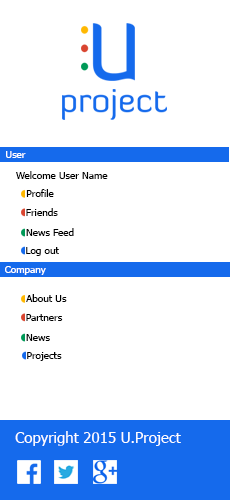
\includegraphics[\linewidth, height=5cm]{Mobile.png} 

\caption{layout do Menu}

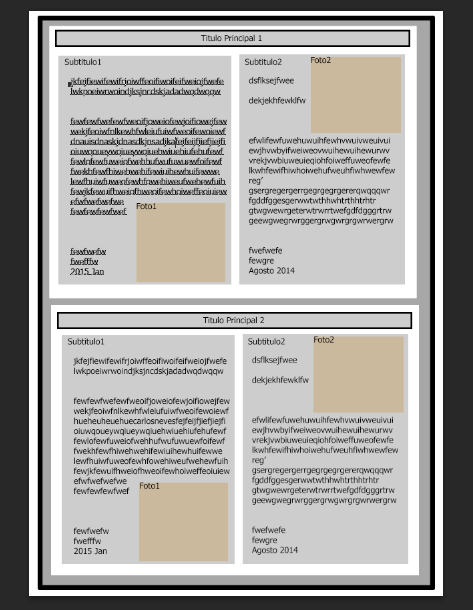
\includegraphics[\linewidth, height=5cm]{Noticias.PNG} 

\caption{layout das noticias}

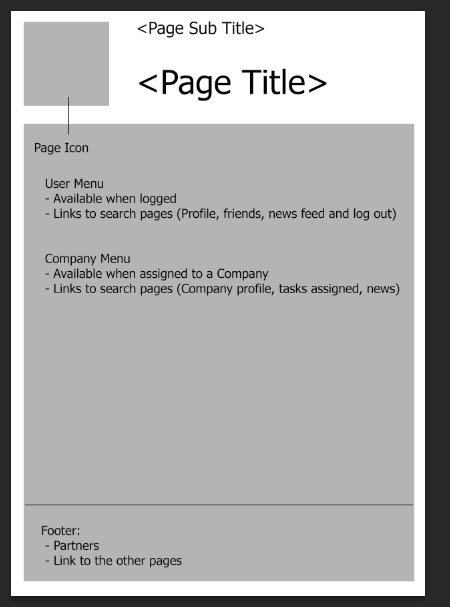
\includegraphics[\linewidth, height=5cm]{Pagina.PNG} 

\caption{layout do utilizador}

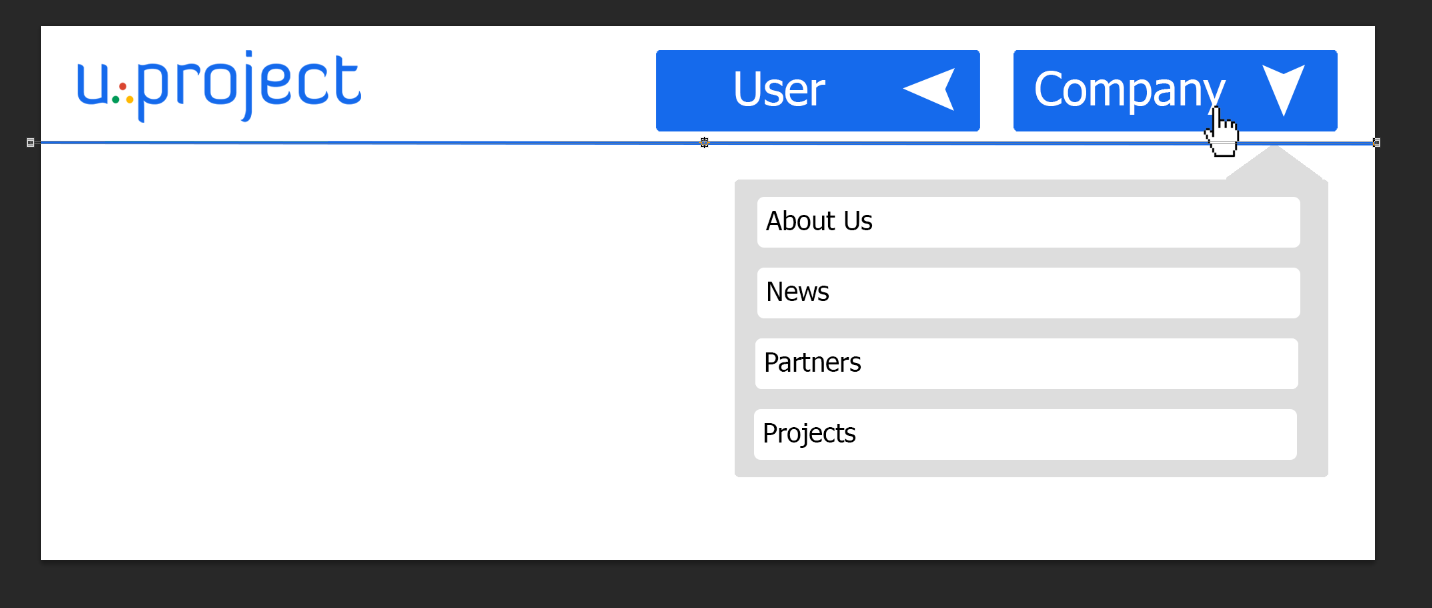
\includegraphics[\linewidth, height=5cm]{Pc.PNG} 

\caption{Coisas}




\subsection{A3B}
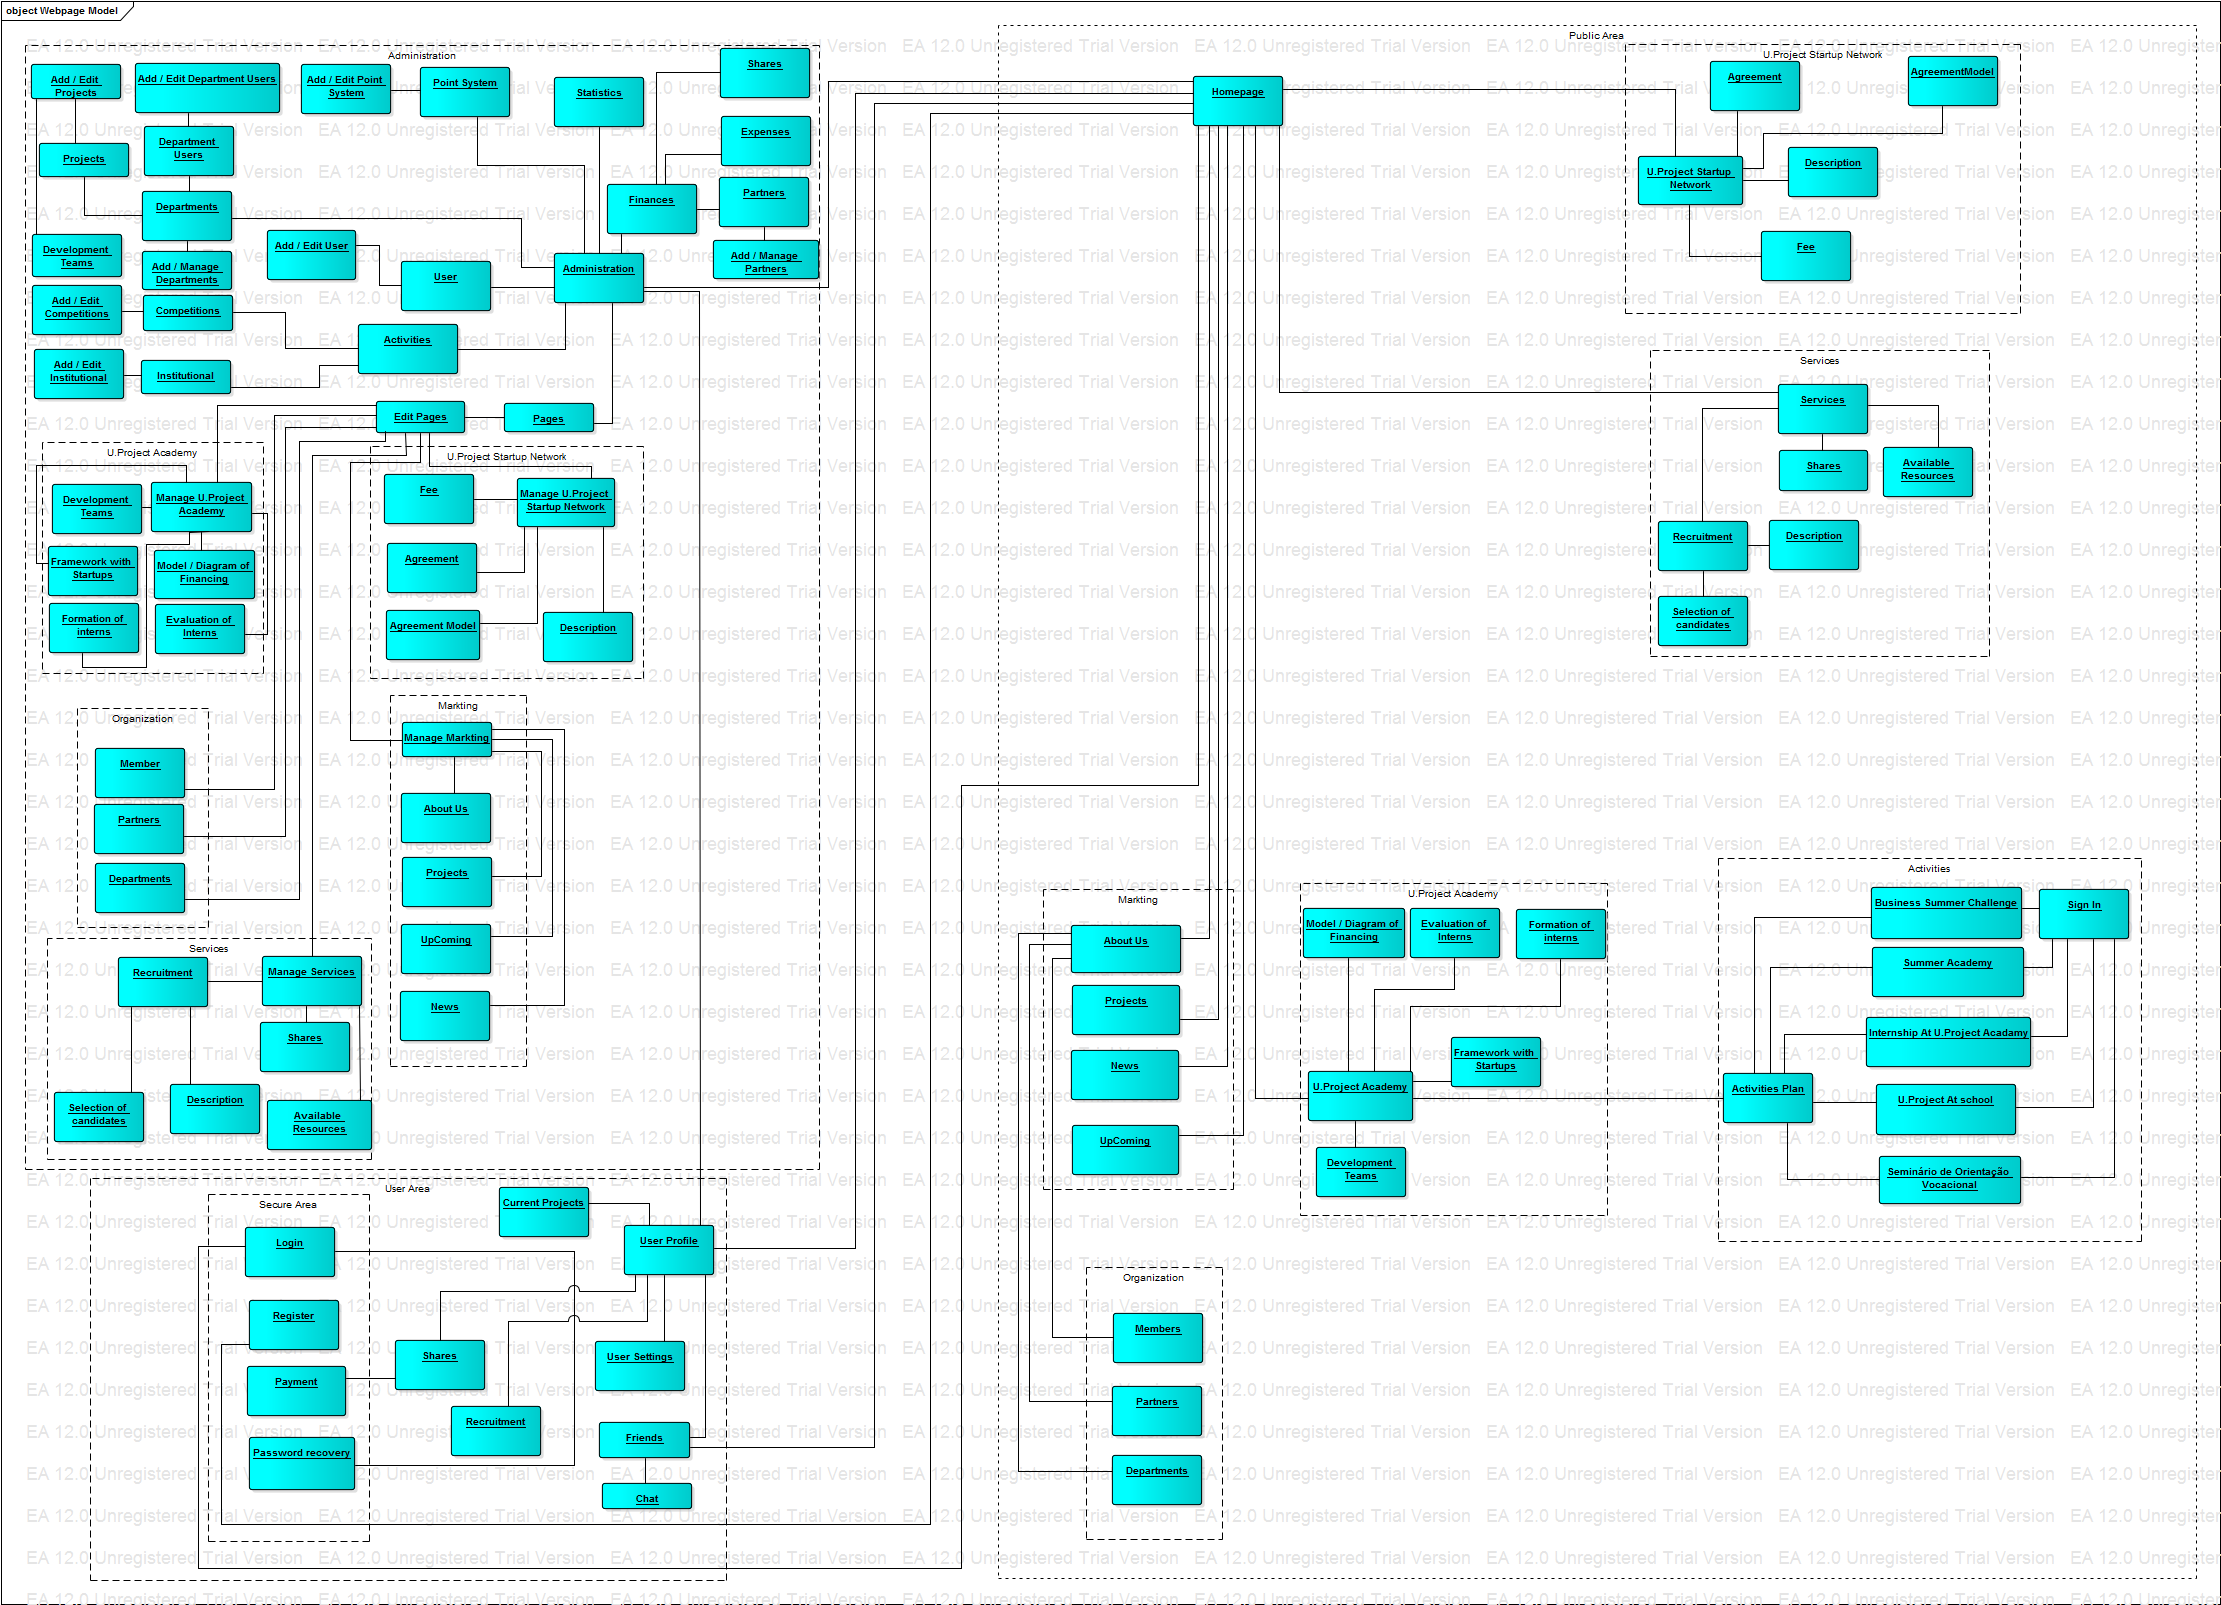
\includegraphics[width=1\linewidth, height=10cm]{Webpage_Model.png} 

\caption{Website Webpage Model}

\subsection{A3C}

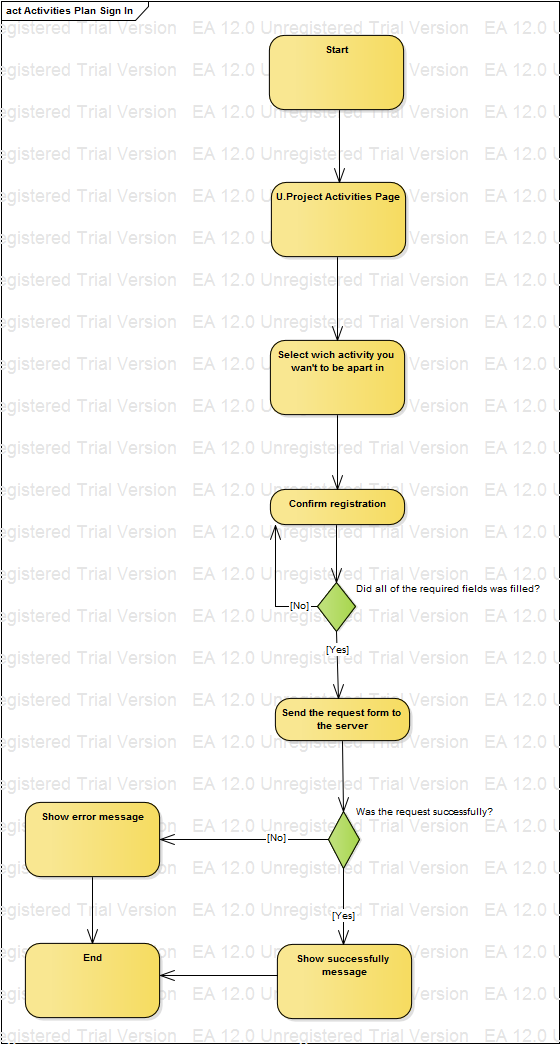
\includegraphics[\linewidth, height=10cm]{Activities_Plan_Sign_In.png} 

\caption{Inscrever-se nas atividades}


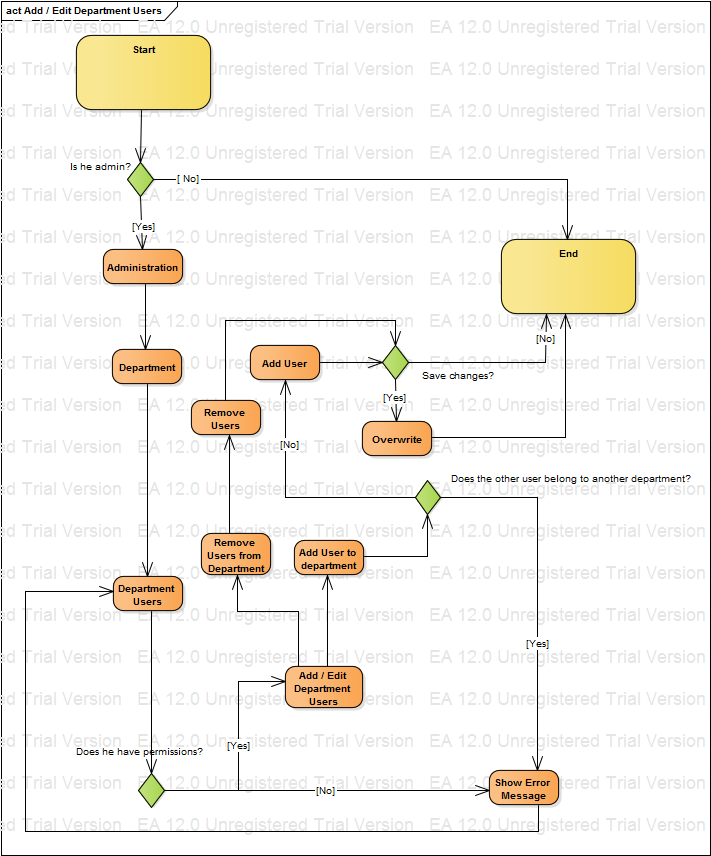
\includegraphics[\linewidth, height=5cm]{Add_Edit_Department_Users.png} 

\caption{Departamento dos Utilizadores}

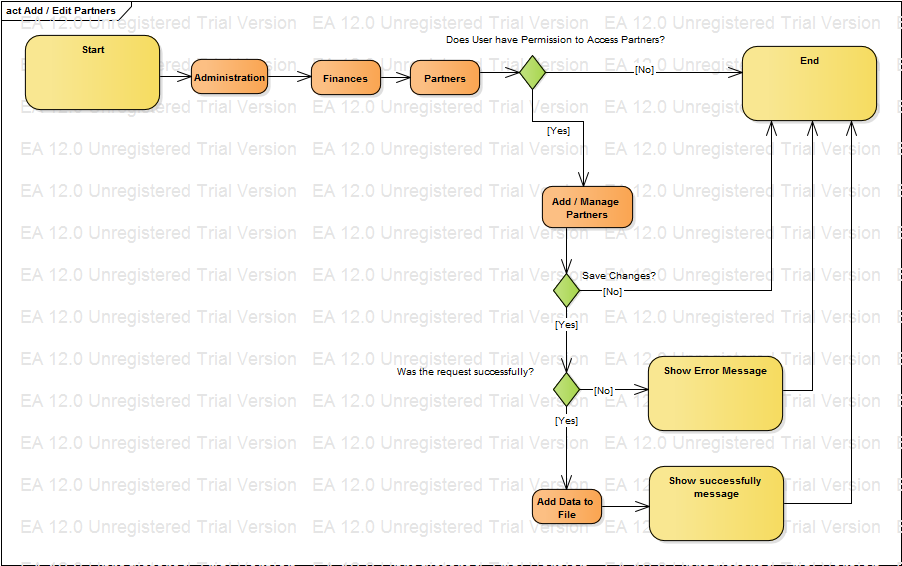
\includegraphics[\linewidth, height=5cm]{Add_Edit_Partners.png} 

\caption{Parceiros}

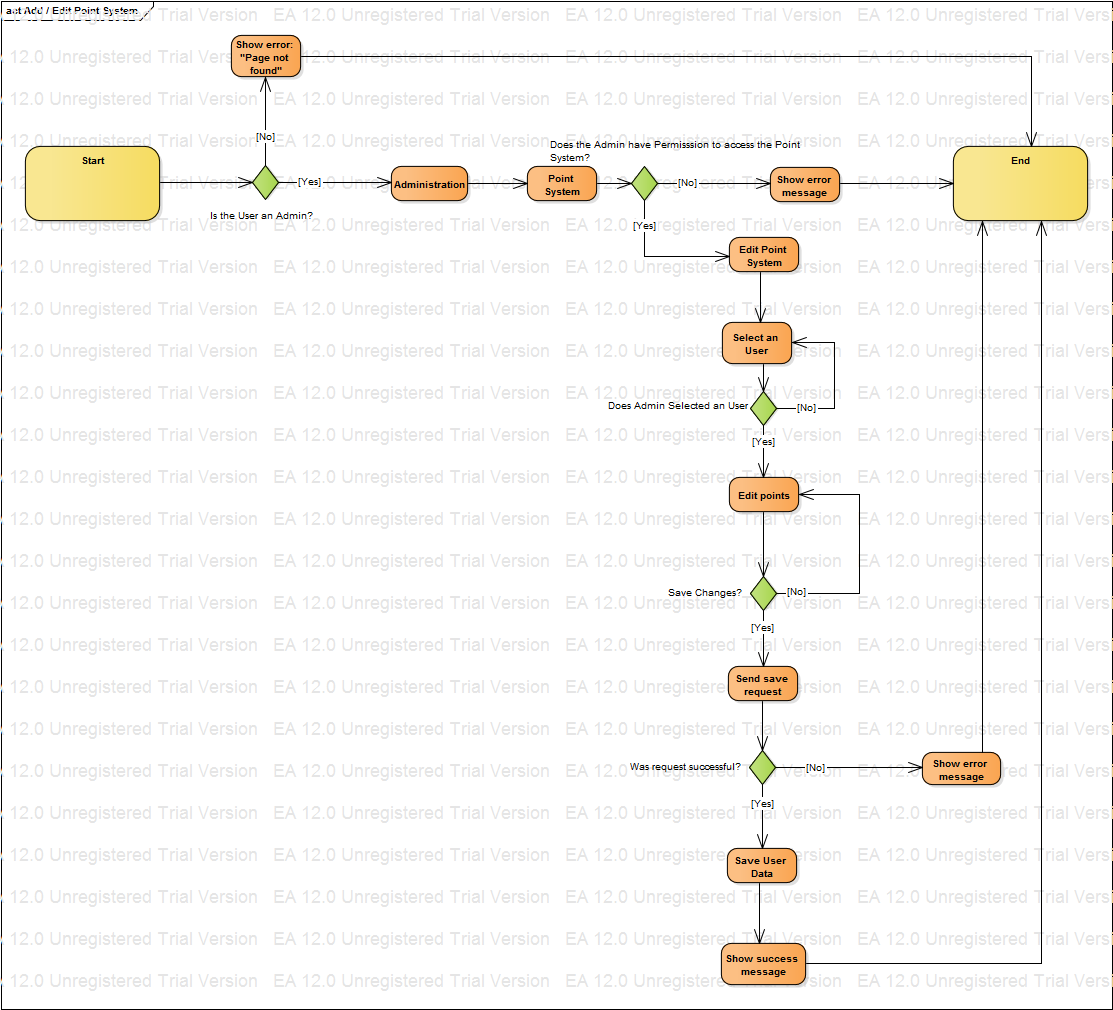
\includegraphics[\linewidth, height=5cm]{Add_Edit_Point_System.png} 

\caption{Sistema de pontos}

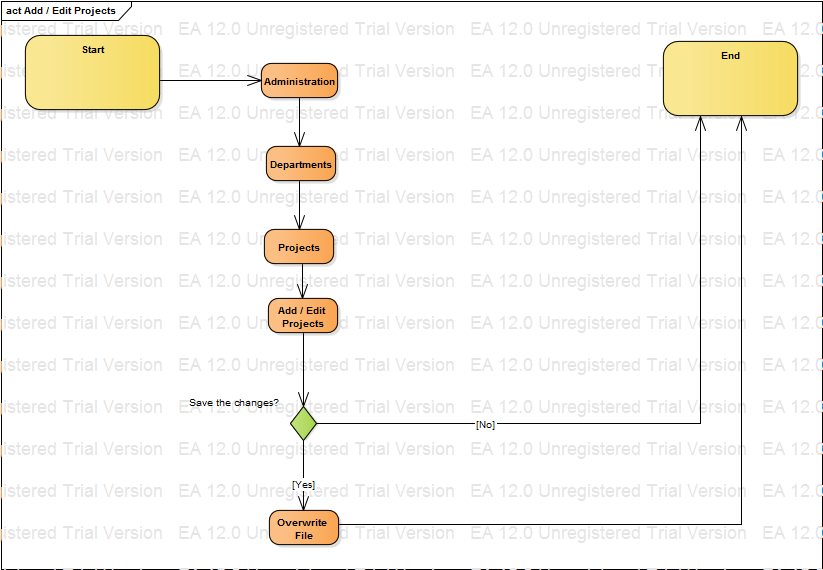
\includegraphics[\linewidth, height=5cm]{Add_Edit_Projects.png} 

\caption{Projetos}

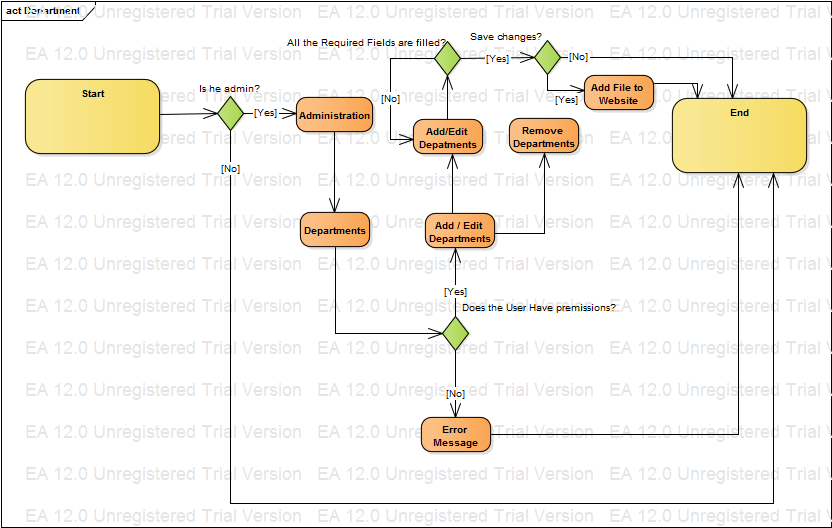
\includegraphics[\linewidth, height=5cm]{Department.png} 

\caption{Departamentos}

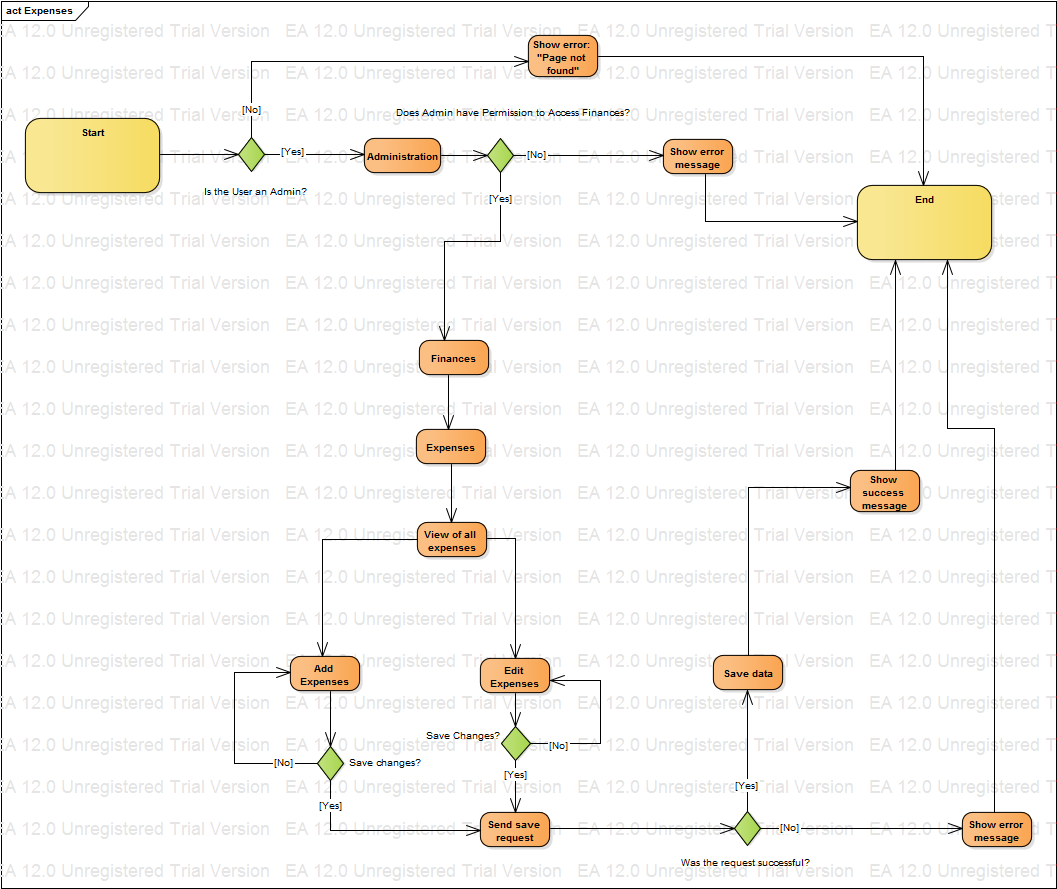
\includegraphics[\linewidth, height=5cm]{Expenses.png} 

\caption{Despesas}

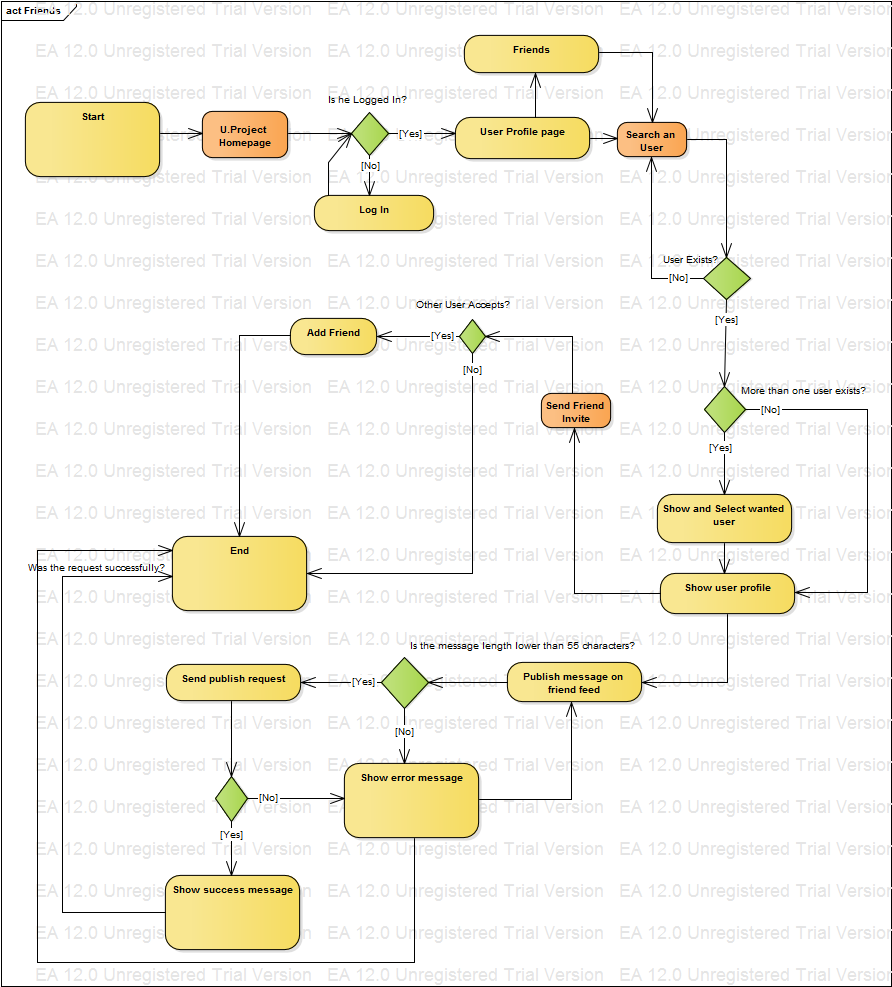
\includegraphics[\linewidth, height=5cm]{Friends.png} 

\caption{Amigos}

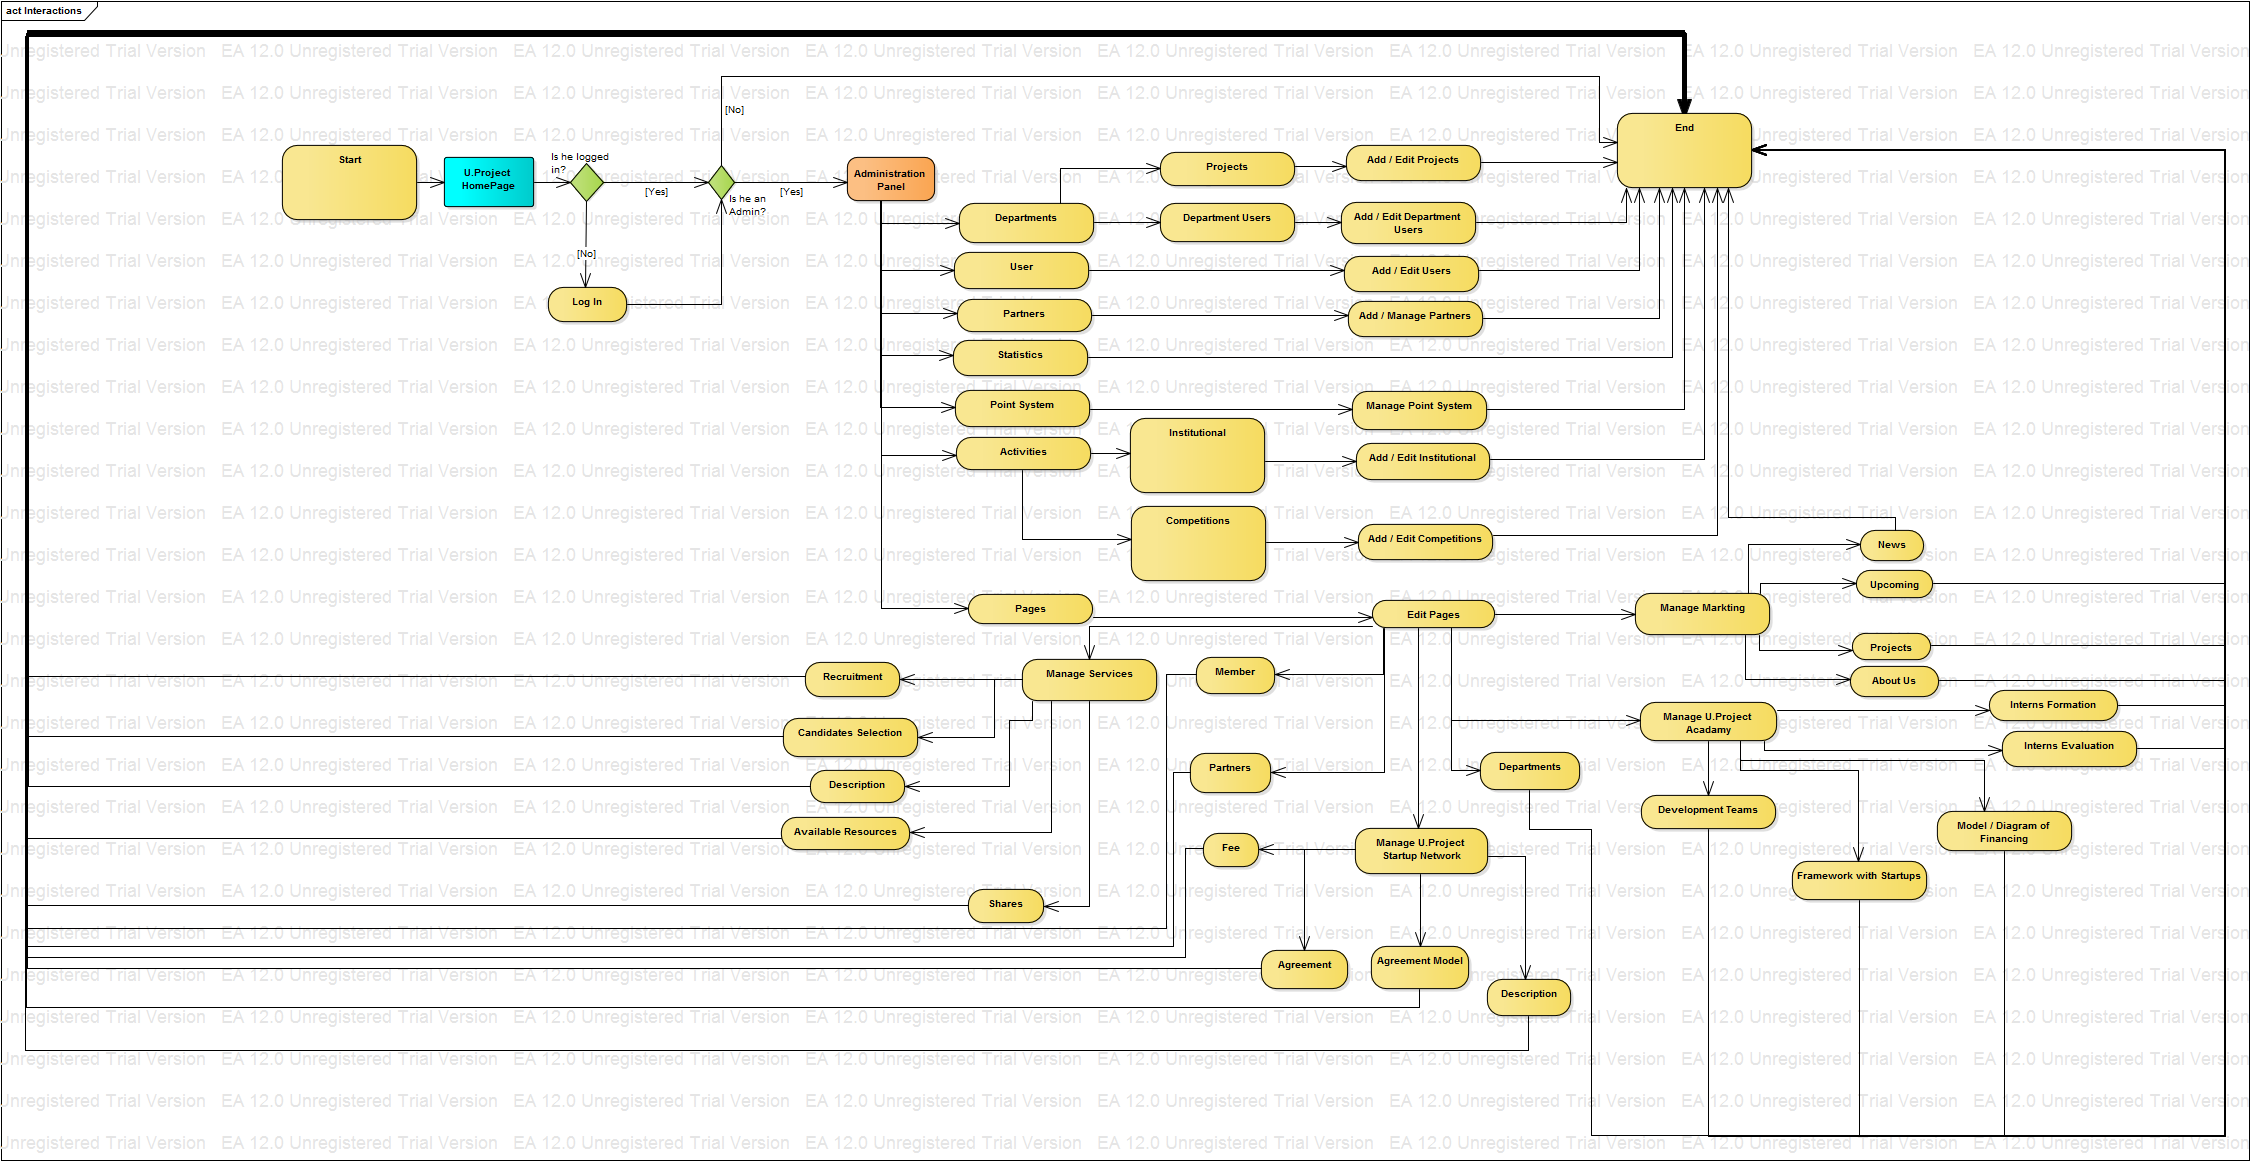
\includegraphics[\linewidth, height=5cm]{Interactions.png} 

\caption{Administração}

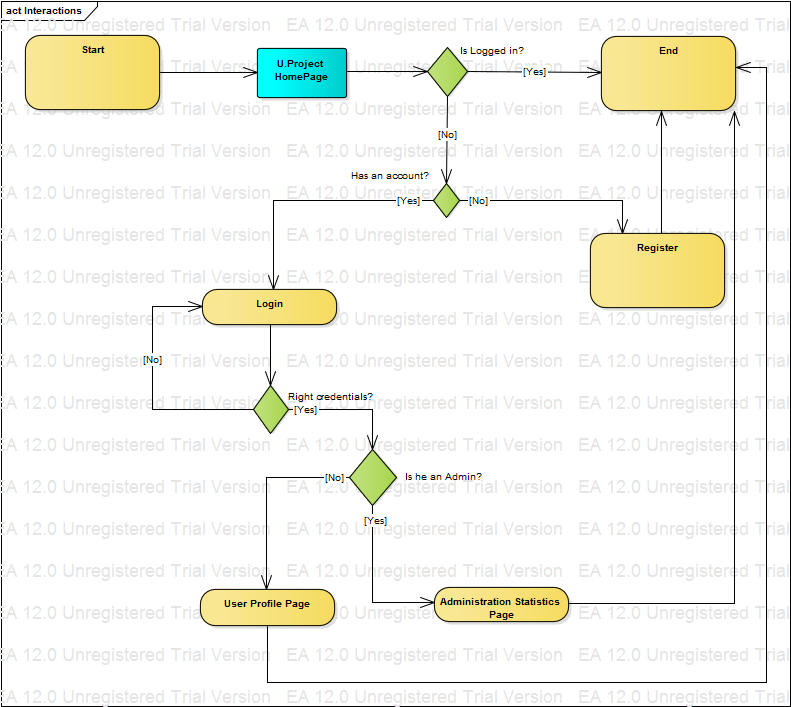
\includegraphics[\linewidth, height=5cm]{Login.png} 

\caption{Iniciar sessão}

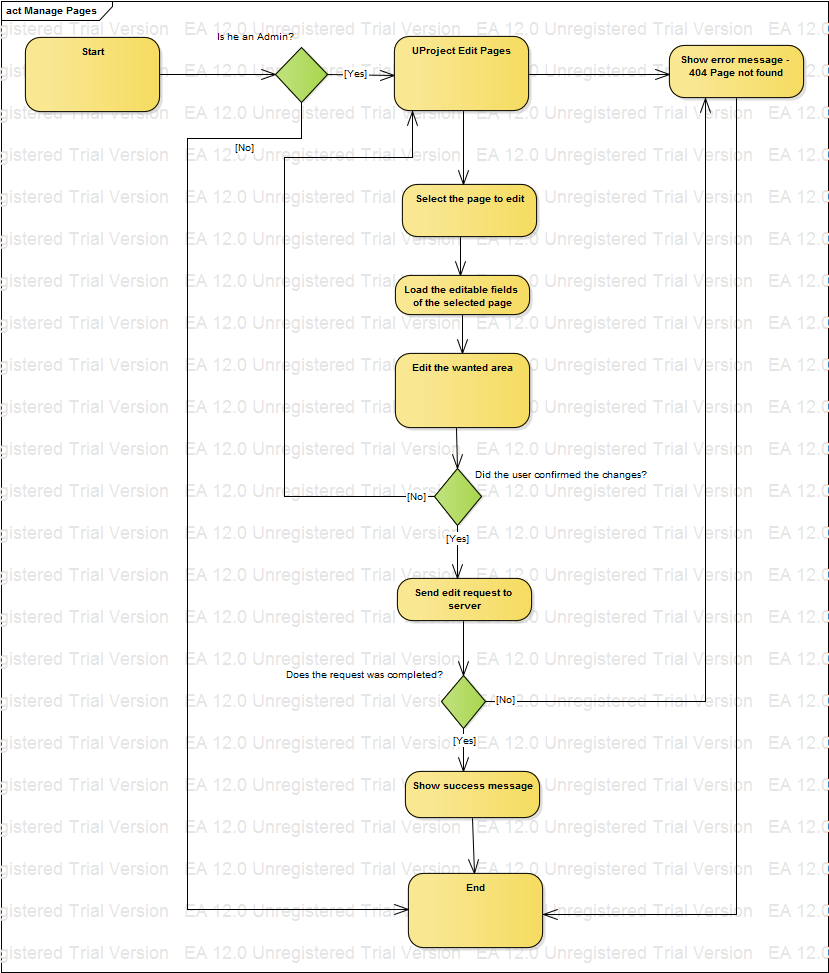
\includegraphics[\linewidth, height=5cm]{Manage_Pages.png} 

\caption{Gestão das paginas}

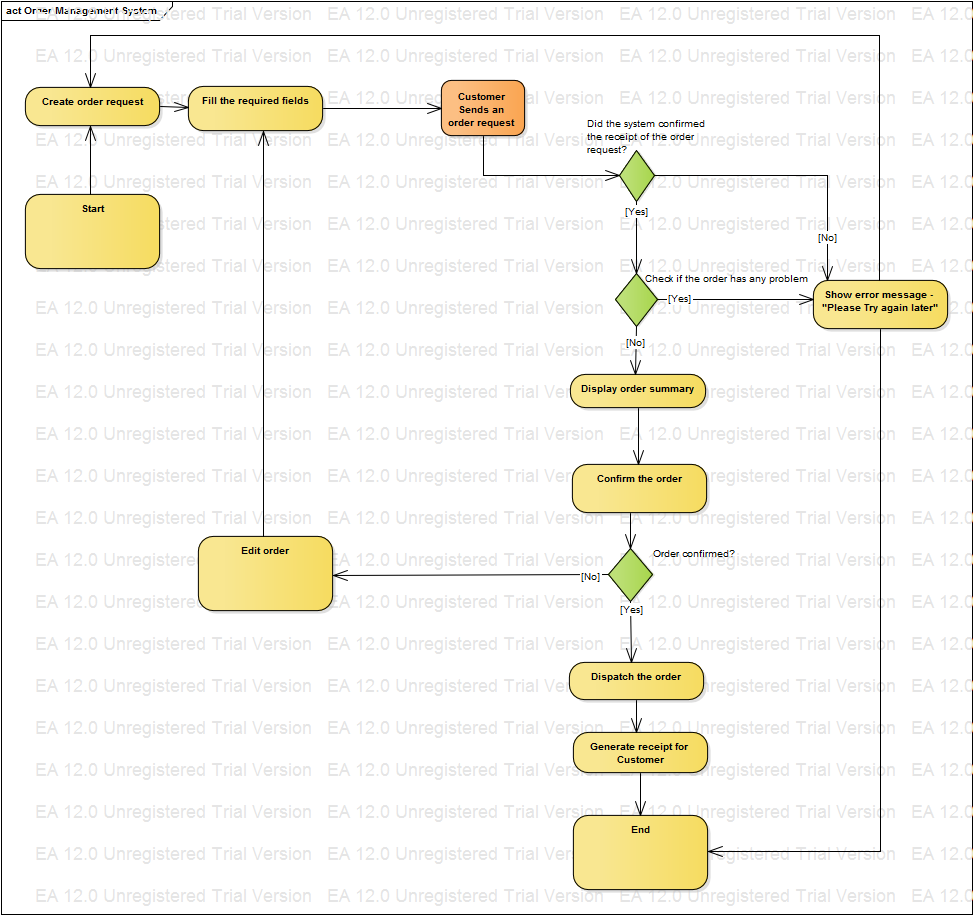
\includegraphics[\linewidth, height=5cm]{Order_Management_System.png} 

\caption{Sistema de gestão}

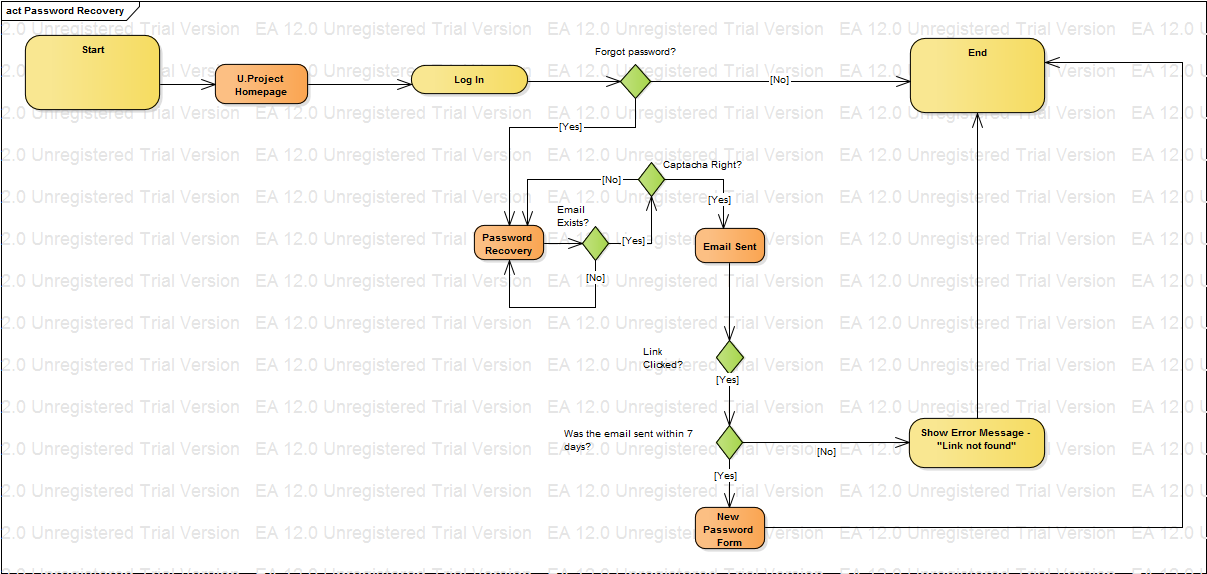
\includegraphics[\linewidth, height=5cm]{Password_Recovery.png} 

\caption{Recuperação da password}

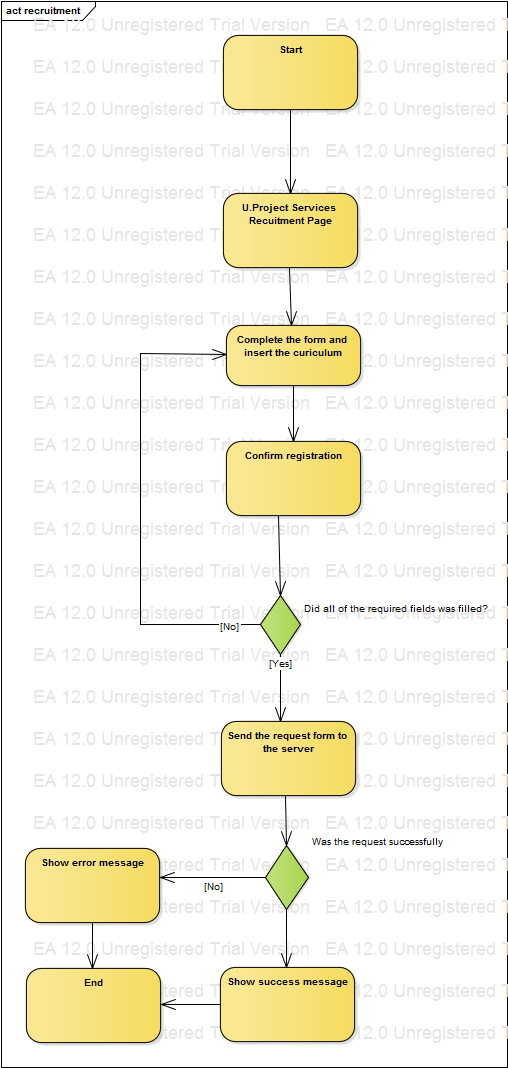
\includegraphics[\linewidth, height=5cm]{recruitment.png} 

\caption{Recrutamento}

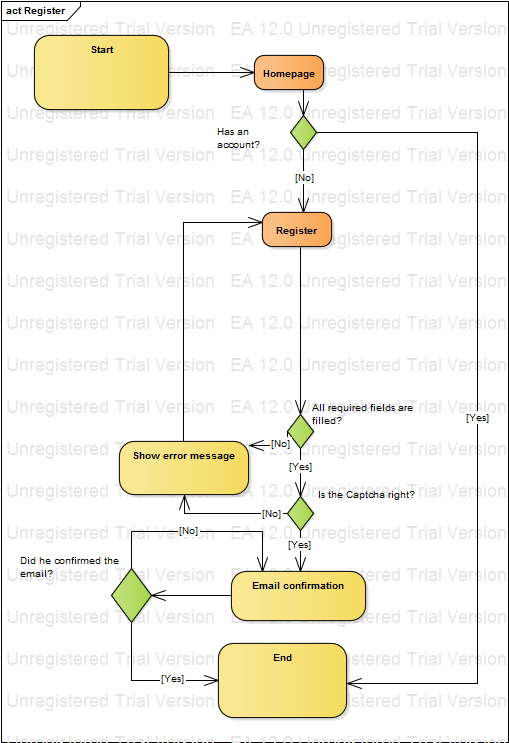
\includegraphics[\linewidth, height=5cm]{Register.png} 

\caption{Resgitar}

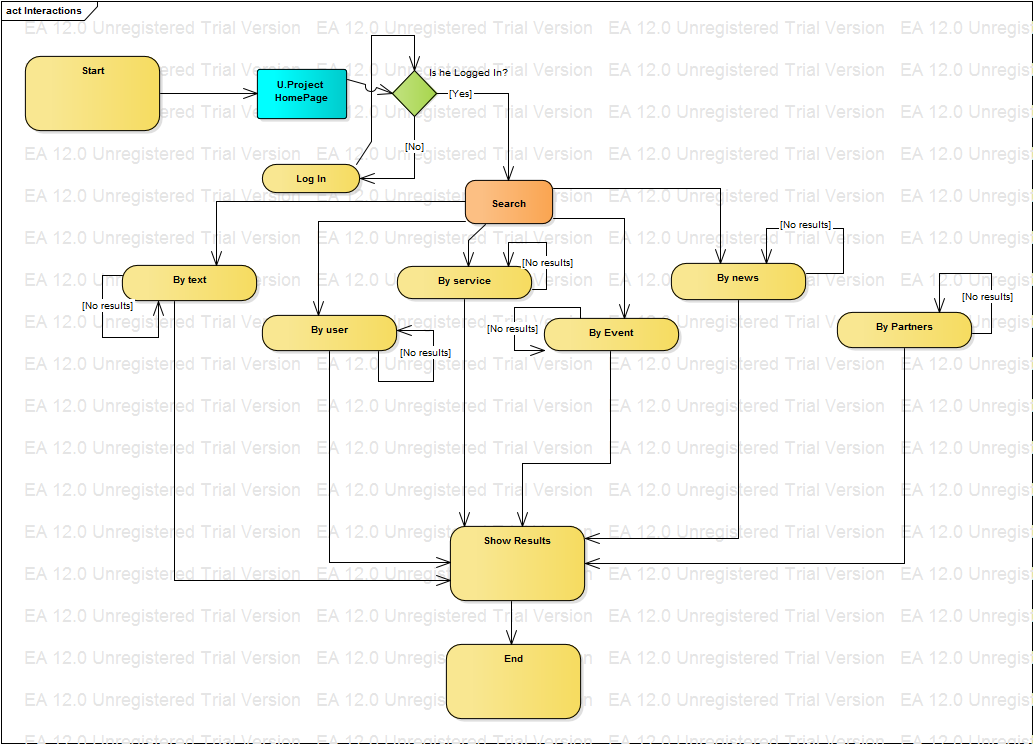
\includegraphics[\linewidth, height=5cm]{Search.png} 

\caption{Pesquisa}

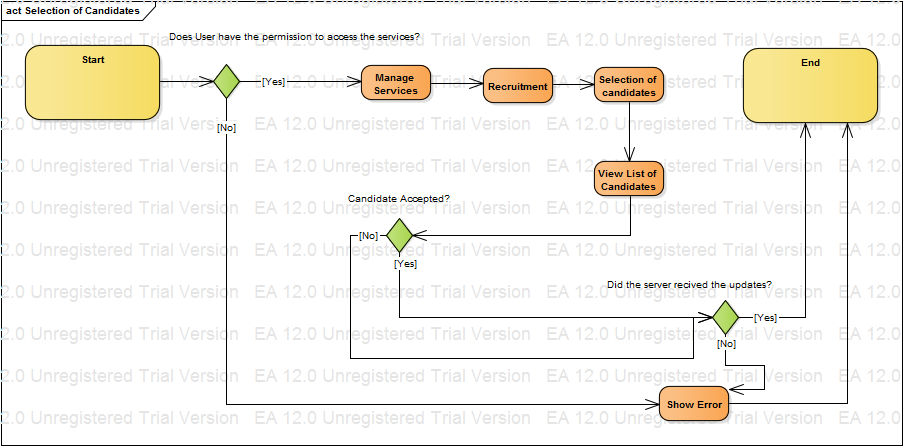
\includegraphics[\linewidth, height=5cm]{Selection_of_Candidates.png} 

\caption{Seleção dos canidatos}

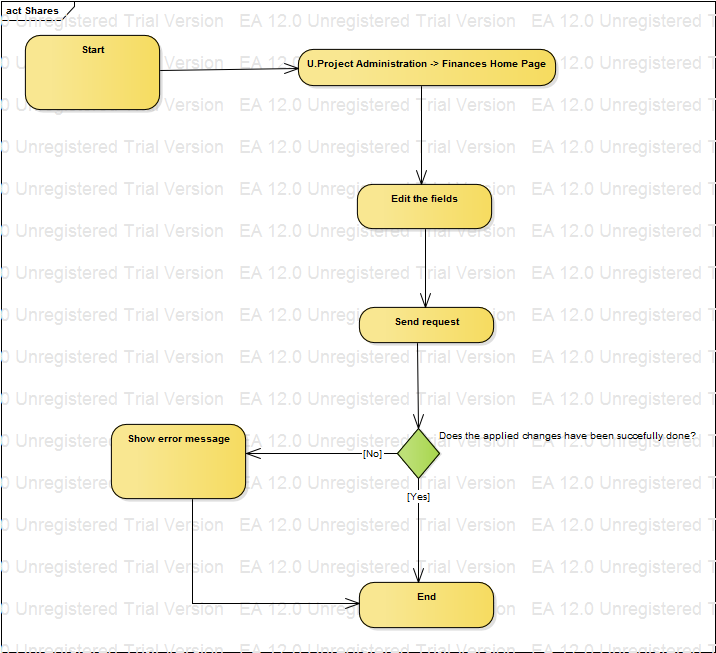
\includegraphics[\linewidth, height=5cm]{Shares.png} 

\caption{Quotas}

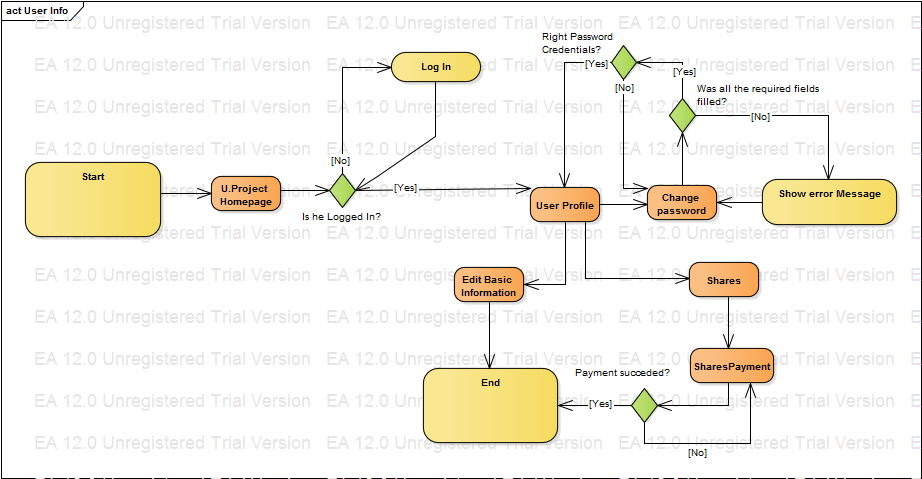
\includegraphics[\linewidth, height=5cm]{User_Info.png} 

\caption{Info do utilizador}

\subsection{A4}

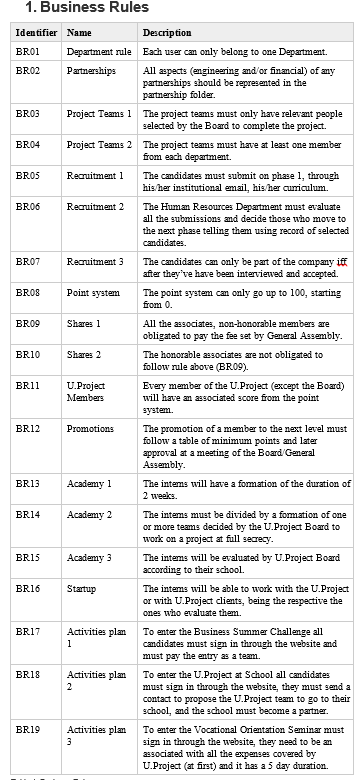
\includegraphics[\linewidth, height=5cm]{Business_rules.PNG} 

\caption{Regras de negócio}

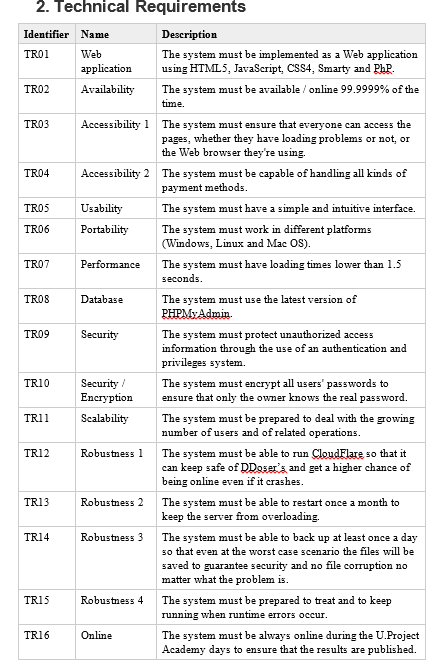
\includegraphics[\linewidth, height=5cm]{Technical_req.PNG} 

\caption{Requerimentos técnicos}

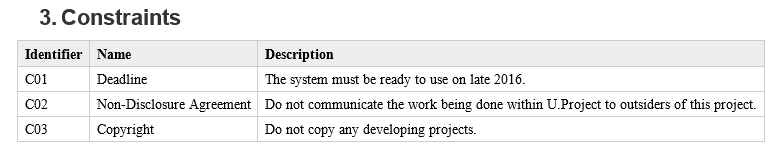
\includegraphics[width=1\linewidth]{Constraints.PNG} 

\caption{Restrições}


\subsection{A5}
\caption{Modelo UMl}
\linebreak
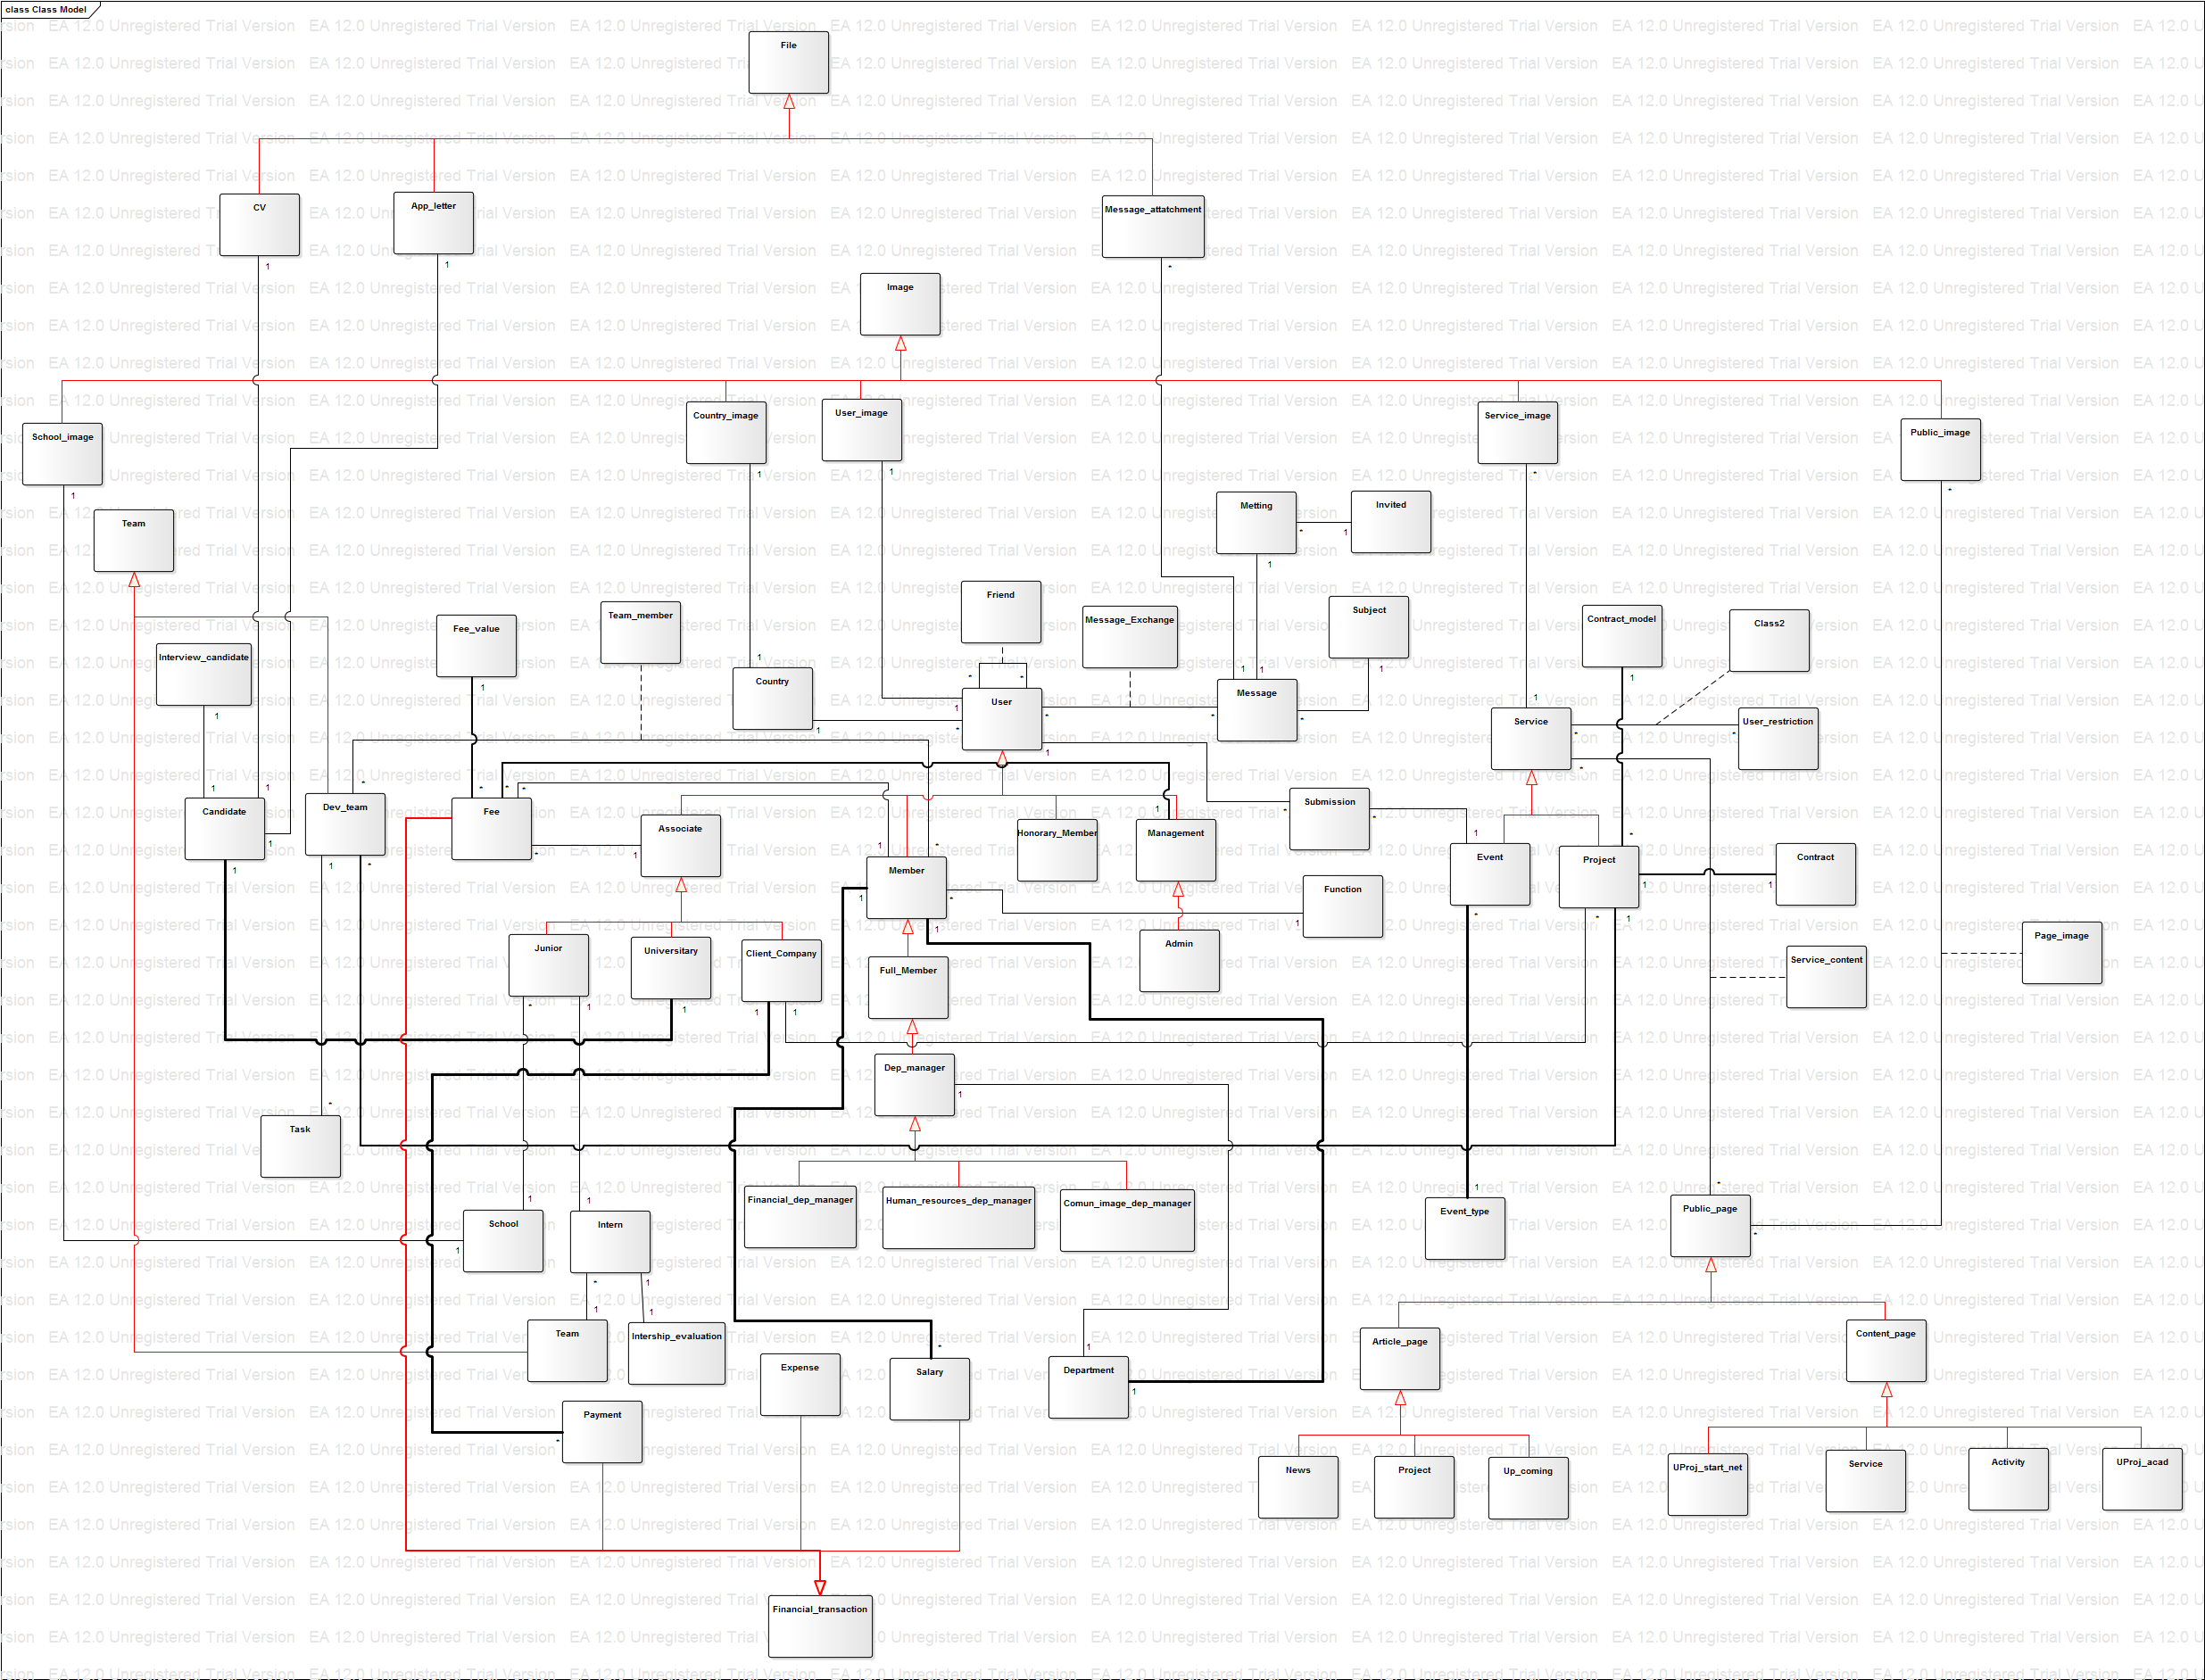
\includegraphics[width=1\linewidth]{Class_Model.png} 
\end{document}